\documentclass[11pt]{amsart}
%\linespread{1.25}
\usepackage[margin=3.5cm]{geometry}

\usepackage[noend,boxruled]{algorithm2e}
%Customize appearance using line below:
\SetKwFor{For}{\normalfont{for}}{:}{endfor}

\usepackage[english]{babel}
\usepackage{appendix}
\usepackage{amsmath}
\usepackage{amsfonts}
\usepackage{amssymb}
%\usepackage{showlabels}
\usepackage{hyperref}
\usepackage{amsthm}
\usepackage{marginnote}
\usepackage{stmaryrd}
\usepackage{enumitem}
\usepackage[english]{babel}
\usepackage{yfonts}
\usepackage[T1]{fontenc}
\usepackage[utf8x]{inputenc}

\usepackage{calrsfs}
\DeclareMathAlphabet{\pazocal}{OMS}{zplm}{m}{n}

\usepackage{verbatim}
\usepackage{graphicx}
\usepackage{verbatim}
\usepackage{faktor}
\usepackage{xcolor}
\usepackage{xfrac}
\usepackage{tikz,tikz-cd}
\usetikzlibrary{decorations.pathmorphing,decorations.pathreplacing,patterns}

\usepackage[all]{xy}
\usepackage{bbm}
\usepackage{tabularx}
\usepackage{longtable}
\usepackage{tabu}
\usepackage{booktabs}
\usepackage{mathtools}

\usepackage[]{textcomp}
\usepackage[sups]{Baskervaldx}
\usepackage{cabin}
\usepackage[varqu,varl]{inconsolata}
\usepackage[baskervaldx,bigdelims,vvarbb]{newtxmath}
\usepackage[cal=cm]{mathalfa}


\newcommand{\plC}{\scalebox{0.8}[1.3]{$\sqsubset$}}
\newcommand{\sidenote}[1]{\marginpar{\textbf{\color{red}#1}}}

% FIGURES FOR USE LATER
%%%%%%%%%%%%%%%%%%%%%%%%%%%%%%%%%%%%%%%%%%%%%%%%%%%%%%%%%%%%
\def\Yagraph{\tikz[baseline=-3pt,scale=.8]{
\draw (2,0) -- (0,1) (2,0) -- (0,.5) (2,0) -- (0,-1);
\draw (2,0) circle(2pt)[fill=black];
\draw [->] (2,0) -- (2.7,0);
\draw (2.6,0) node[right]{\tiny{$x_k$}};
\draw (0,1) circle(2pt)[fill=white];
\draw (0,.5) circle(2pt)[fill=black];
\draw (0,-.25) node{$\vdots$};
\draw (0,-1) circle(2pt)[fill=black];
\draw [red,fill=red] (0,-2) circle[radius=2pt];
\draw [->,red,thick] (0,-2) -- (2,-2);
\draw (2,-2) node[right,red]{\tiny{$\Sigma(\PP^N|H)$}};
\draw [->,red] (1,-0.9) -- (1,-1.6);

\draw (2.05,0) node[above]{\tiny{$\sqC_0$}};
\draw (0,1) node[left]{\tiny{$\sqC_1$}};
\draw (0,.5) node[left]{\tiny{$\sqC_2$}};
\draw (0,-1) node[left]{\tiny{$\sqC_r$}};
}}

\def\Ybgraph{\tikz[baseline=-3pt,scale=.8]{
\draw (2,0) to[out=120,in=0] (0,1) (2,0) -- (0,1) (2,0) -- (0,.5) (2,0) -- (0,-1);
\draw (2,0) circle(2pt)[fill=black];
\draw [->] (2,0) -- (2.7,0);
\draw (2.6,0) node[right]{\tiny{$x_k$}};
\draw (0,1) circle(2pt)[fill=black];
\draw (0,.5) circle(2pt)[fill=black];
\draw (0,-.25) node{$\vdots$};
\draw (0,-1) circle(2pt)[fill=black];
\draw [red,fill=red] (0,-2) circle[radius=2pt];
\draw [->,red,thick] (0,-2) -- (2,-2);
\draw (2,-2) node[right,red]{\tiny{$\Sigma(\PP^N|H)$}};
\draw [->,red] (1,-0.9) -- (1,-1.6);

\draw (2.05,0) node[above]{\tiny{$\sqC_0$}};
\draw (0,1) node[left]{\tiny{$\sqC_1$}};
\draw (0,.5) node[left]{\tiny{$\sqC_3$}};
\draw (0,-1) node[left]{\tiny{$\sqC_r$}};
}}

\def\Ycgraph{\tikz[baseline=-3pt,scale=.8]{
\draw (2,0) -- (0,1) (2,0) -- (0,.5) (2,0) -- (0,-1);
\draw [->] (2,0) -- (2.7,0);
\draw (2.6,0) node[right]{\tiny{$x_k$}};
\draw (2,0) circle(2pt)[fill=white];
\draw (0,1) circle(2pt)[fill=black];
\draw (0,.5) circle(2pt)[fill=black];
\draw (0,-.25) node{$\vdots$};
\draw (0,-1) circle(2pt)[fill=black];
\draw [red,fill=red] (0,-2) circle[radius=2pt];
\draw [->,red,thick] (0,-2) -- (2,-2);
\draw (2,-2) node[right,red]{\tiny{$\Sigma(\PP^N|H)$}};
\draw [->,red] (1,-0.9) -- (1,-1.6);

\draw (2.05,0) node[above]{\tiny{$\sqC_0$}};
\draw (0,1) node[left]{\tiny{$\sqC_1$}};
\draw (0,.5) node[left]{\tiny{$\sqC_2$}};
\draw (0,-1) node[left]{\tiny{$\sqC_r$}};
}}
%%%%%%%%%%%%%%%%%%%%%%%%%%%%%%%%%%%%%%%%%%%%%%%%%%%%%%%%%%%%%%

\newcommand{\mathsq}[1]{#1}

\newcommand{\sqC}{\scalebox{0.8}[1.3]{$\sqsubset$}}

\newcommand{\pM}{\pazocal{M}}
\newcommand{\TT}{\operatorname{T}}
\newcommand{\oM}{\overline{\mathcal{M}}}
\newcommand{\M}[4]{\overline{\mathcal{M}}_{#1,#2}(#3,#4)}

\newcommand{\Mlog}[4]{\overline{\mathcal{M}}^{\operatorname{log}}_{#1,#2}(#3,#4)}
\newcommand{\MLog}{\overline{\mathcal{M}}^{\operatorname{log}}}
\newcommand{\Mpunct}[4]{\overline{\mathcal{M}}^{\operatorname{punct}}_{#1,#2}(#3,#4)}
\newcommand{\MG}[4]{\overline{\mathcal{M}}^{\rm G}_{#1,#2}(#3,#4)}
\newcommand{\Q}[4]{\mathcal{Q}_{#1,#2}(#3,#4)}
\newcommand{\Qe}[4]{\mathcal{Q}^{\epsilon}_{#1,#2}(#3,#4)}
\newcommand{\Qt}[4]{\widetilde{\mathcal Q}_{#1,#2}(#3,#4)}
\newcommand{\QG}[4]{\mathcal{Q}G_{#1,#2}(#3,#4)}
\newcommand{\QGe}[4]{\mathcal{Q}G^{\epsilon}_{#1,#2}(#3,#4)}
\newcommand{\D}[3]{\mathcal{D^Q}(#1,#2,#3)}
\newcommand{\E}[3]{\mathcal{E^Q}(#1,#2,#3)}
\newcommand{\PP}{\mathbb P}
\newcommand{\Z}{\mathbb{Z}}
\newcommand{\VZ}{\pazocal{V\!Z}}
\newcommand{\tVZc}[4]{\widetilde{\mathcal{V\!Z}}^{\rm{ctr}}_{#1,#2}(#3,#4)}
\newcommand{\VZc}[4]{\mathcal{V\!Z}_{#1,#2}(#3,#4)}
\newcommand{\VZcLi}[4]{\mathcal{V\!Z}^{\rm{ctr, Li}}_{#1,#2}(#3,#4)}
\newcommand{\VZrel}[4]{\mathcal{V\!Z}^{\rm{rel}}_{#1,#2}(#3,#4)}
\newcommand{\stab}{\rm{stab}}
\newcommand{\st}{\star}
\newcommand{\stC}{C'}
\newcommand{\stpi}{\pi'}
\newcommand{\sts}{s'}
\newcommand{\N}{\mathbb{N}}
\newcommand{\OO}{\mathcal{O}}
\renewcommand{\to}{\rightarrow}
\newcommand{\A}{\mathcal A}
\newcommand{\B}{\mathcal B}
\newcommand{\C}{\mathfrak C}
\newcommand{\cC}{\mathcal C}
\newcommand{\EE}{\mathbf{E}}
\renewcommand{\L}{\mathcal L}
\newcommand{\LL}{\mathbf{L}}
\newcommand{\MM}{\mathfrak M}
\newcommand{\Aaff}{\mathbb{A}}
\newcommand{\kfield}{\Bbbk}
\newcommand{\comp}{\chi}
\newcommand{\sst}{\sigma^{\operatorname{ss}}}
\newcommand{\Pic}{\operatorname{Pic}}
\newcommand{\Def}{\operatorname{Def}}
\newcommand{\Spec}{\operatorname{Spec}}
\newcommand{\Proj}{\operatorname{Proj}}
\newcommand{\Hom}{\operatorname{Hom}}
\newcommand{\Ext}{\operatorname{Ext}}
\newcommand{\Gm}{\mathbb{G}_{\text{m}}}
\newcommand{\virt}[1]{[#1]^{\operatorname{virt}}}
\newcommand{\vip}[1]{[#1]^{\operatorname{prod}}}
\newcommand{\Id}{\operatorname{Id}}
\newcommand{\CC}{\mathbb{C}}
\newcommand{\QQ}{\mathbb{Q}}
\newcommand{\HH}{\operatorname{H}}
\newcommand{\Achow}{\operatorname{A}}
\newcommand{\pt}{\operatorname{pt}}
\newcommand{\bq}{\begin{equation}}
\newcommand{\eq}{\end{equation}}
\newcommand{\ba}{\begin{aligned}}
\newcommand{\ea}{\end{aligned}}
\newcommand{\be}{\begin{enumerate}}
\newcommand{\ee}{\end{enumerate}}
\newcommand{\bsm}{\left(\begin{smallmatrix}}
\newcommand{\esm}{\end{smallmatrix}\right)}                   
\newcommand{\bpm}{\begin{pmatrix}}
\newcommand{\epm}{\end{pmatrix}}
\newcommand{\barr}{\begin{displaymath}\begin{array}{cccc}}
\newcommand{\earr}{\end{array}\end{displaymath}}
\newcommand{\barrl}{\begin{displaymath}\begin{array}{lcl}}
\newcommand{\earrl}{\end{array}\end{displaymath}}
\newcommand{\barl}{\begin{displaymath}\begin{array}{l}}
\newcommand{\earl}{\end{array}\end{displaymath}}
\newcommand{\bxym}{ \begin{displaymath}\xymatrix }
\newcommand{\exym}{\end{displaymath}}
\newcommand{\bcd}{\begin{center}\begin{tikzcd}}
\newcommand{\ecd}{\end{tikzcd}\end{center}}
\newcommand{\R}{\operatorname{R}^{\bullet}}
\newcommand{\dvr}{\Delta}
%\newcommand{\sslash}{\mathbin{/\mkern-6mu/}}
\newcommand{\tr}{{\rm tr}}
\newcommand{\Isom}{\text{Isom}}
\newcommand{\pr}{\operatorname{pr}}
\newcommand{\ev}{\operatorname{ev}}
\newcommand{\fgt}{\operatorname{fgt}}
\newcommand{\codim}{\operatorname{codim}}
\newcommand{\vdim}{\operatorname{vdim}}
\newcommand{\ildef}[1]{\emph{#1}}
\newcommand{\om}[1]{\mathcal{#1}}
\newcommand{\h}{\operatorname{h}}
\newcommand{\Aut}{\operatorname{Aut}}
\newcommand{\Acal}{\mathcal{A}}
\newcommand{\Scal}{\mathcal{S}}
\newcommand{\Mcal}{\mathcal{M}}
\newcommand{\Dcal}{\mathcal{D}}
\newcommand{\Ncal}{\mathcal{N}}
\newcommand{\Lcal}{\mathcal{L}}
\newcommand{\Ccal}{\mathcal{C}}
\newcommand{\Pcal}{\mathcal{P}}
\newcommand{\Ycal}{\mathcal{Y}}
\newcommand{\cchern}{\mathrm{c}}
\newcommand{\ol}[1]{\overline{#1}}
\newcommand{\ul}[1]{\underline{#1}}
\newcommand{\op}[1]{\operatorname{#1}}
\newcommand{\gp}{\operatorname{gp}}
\newcommand{\RR}{\mathbb{R}}
\newcommand{\NN}{\mathbb{N}}
\newcommand{\ovm}[1]{\overline{\mathcal{#1}}}
\newcommand{\ovt}[1]{\widetilde{\mathcal{#1}}}
\newcommand{\ov}[1]{\overline{#1}}

\theoremstyle{definition}
\newtheorem{thm}{Theorem}[section]
\newtheorem{lem}[thm]{Lemma}
\newtheorem{lemma}[thm]{Lemma}
\newtheorem{prop}[thm]{Proposition}
\newtheorem{cor}[thm]{Corollary}
\newtheorem*{teo*}{Theorem}
\newtheorem{ipotesi}{ipotesi}
\newtheorem*{nota}{Nota}
\newtheorem{claim}{Claim}
\newtheorem{question}[thm]{Question}
\newtheorem{conj}[thm]{Conjecture}
\newtheorem{notation}[thm]{Notation}

\newtheorem{innercustomthm}{Theorem}
\newenvironment{customthm}[1]
  {\renewcommand\theinnercustomthm{#1}\innercustomthm}
  {\endinnercustomthm}

\theoremstyle{definition}
\newtheorem{example}[thm]{Example}
\newtheorem{ex}[thm]{Example}
\newtheorem{dfn}[thm]{Definition}
\newtheorem{definition}[thm]{Definition}
\newtheorem{aside}[thm]{Aside}
\newtheorem{remark}[thm]{Remark}
\newtheorem{com}[thm]{Comment}
\newtheorem{num}{Number}
\newtheorem*{sketch}{Sketch}
\newtheorem*{rem}{Remark}
\newtheorem*{aside*}{Aside}
\newtheorem*{acknowledgements}{Acknowledgements}

\newlist{steps}{enumerate}{1}
\setlist[steps, 1]{label = Step (\arabic*):}

\newcommand{\ilemph}[1]{\emph{#1}}

\setcounter{tocdepth}{1}

\newcommand{\todo}[1]{\vspace{5mm}\par \noindent
\framebox{\begin{minipage}[c]{0.95 \textwidth} \tt #1\end{minipage}} \vspace{5mm} \par}

\def\ti{-\allowhyphens}
\newcommand{\thismonth}{\ifcase\month % case 0 --- impossible!
  \or January\or February\or March\or April\or May\or June%
  \or July\or August\or September\or October\or November%
  \or December\fi}
\newcommand{\thismonthyear}{{\thismonth} {\number\year}}
\newcommand{\thisdaymonthyear}{{\number\day} {\thismonth} {\number\year}}

\title{Gromov--Witten theory of hypersurfaces in genus one}
\author{Luca Battistella, Navid Nabijou and Dhruv Ranganathan}
\date{\thismonthyear}

\begin{document}


\begin{abstract}
\end{abstract}

\maketitle

\appendixtitletocoff
%\tableofcontents

\section{Description of the logarithmic strata}
\noindent Let $\VZ = \VZ_{1,\alpha}(\PP^N|H,d)$ and let $\Acal$ denote the Artin fan of $\VZ$. Since the map of log stacks
\begin{equation*} \VZ \to \Acal \end{equation*}
is smooth, we see that the codimension-$k$ logarithmic strata in $\VZ$ are in bijective correspondence (via pull-back) with the codimension-$k$ logarithmic strata in $\Acal$. The logarithmic strata in $\Acal$, on the other hand, have a purely combinatorial description (at least locally) in terms of the associated moduli spaces of tropical maps, coming from the fact that $\VZ$ is a logarithmic blow-up of the usual moduli space of log stable maps. In this section we discuss this circle of ideas, and show how it plays out in a number of examples.

\subsection{Blowing up the Artin fan}
Let $\Mcal = \ol{\Mcal}^{\op{log}}_{1,\alpha}(\PP^N|H,d)$ denote the Abramovich--Chen--Gross--Siebert moduli space of log stable maps. Recall that $\VZ$ is obtained as a closed substack of a log modification
\begin{equation*} \widetilde{\VZ} \to \Mcal .\end{equation*}
Since the map $\VZ \hookrightarrow \widetilde{\VZ}$ is strict, the Artin fan $\Acal$ of $\VZ$ is locally isomorphic to the Artin fan of $\widetilde{\VZ}$ (with the latter being, in general, larger)\footnote{(Navid) Make this more precise}. Since the following discussion is entirely local, we will ignore the distinction between the two, and pretend as though $\Acal$ is the Artin fan of $\widetilde{\VZ}$. There is then a commuting square:
\bcd
\widetilde{\VZ} \ar[r] \ar[d] & \Mcal \ar[d] \\
\Acal \ar[r] & \Acal_{\Mcal}.
\ecd
Note that neither of the vertical maps are smooth, since the moduli spaces on the top row are not log smooth. The construction of $\widetilde{\VZ} \to \Mcal$ as the log modification obtained by imposing an alignment condition gives us a combinatorial description of the map $\Acal \to \Acal_{\Mcal}$ which we will use to study $\Acal$. Recall that $\Acal_\Mcal$ is locally isomorphic to the stack quotient
\begin{equation*} \left[ \Spec \kfield[Q] / \Spec\kfield [Q^{\gp}] \right]\end{equation*}
where $Q$ is a monoid giving a\footnote{(Navid) Neat?} local chart for $\Mcal$, which we may take to be the minimal monoid of \cite[\S 1.5]{GrossSiebertLog}. The real dual $Q^\vee_{\RR} = \Hom(Q,\RR_{\geq 0})$ of this monoid can be viewed as a moduli space of tropical maps; see \cite[Remark 1.12]{GrossSiebertLog}. We call this \emph{the tropical moduli space}; contained in the tropical moduli space are the edge lengths of the associated tropical curve (corresponding to the smoothing parameters of the nodes of the logarithmic curve). Since the alignment condition amounts to imposing a partial ordering amongst certain sums of these edge lengths, it produces a polyhedral decomposition of the tropical moduli space, into chambers where different partial order relations hold. If we only consider the integral points, this produces a polyhedral decomposition of the cone $Q^\vee = \Hom(Q,\N)$. Dualising, we obtain a toric blow-up
\begin{equation*} Z \to \Spec \kfield[Q] \end{equation*}
which, since it is equivariant, descends to a morphism of the associated zero-dimensional stacks:
\begin{equation*} \left[Z/T_Z \right] \to \left[ \Spec \kfield[Q] / \Spec\kfield [Q^{\gp}] \right]. \end{equation*}
This gives a local description of the map $\Acal \to \Acal_\Mcal$ and in particular of the Artin fan $\Acal$. By the orbit-cone correspondence, the codimension-$k$ strata of $\Acal$ which intersect this open locus correspond to the $k$-dimensional cones in the polyhedral decomposition of $Q^\vee$ described above. These can be understood entirely in terms of tropical combinatorics. This is best explained through a number of examples, which we now present.

\subsection{Examples of logarithmic strata} In these examples we will proceed as follows: we will start by fixing an element of the ordinary moduli space $\Mcal$ of log stable maps. We will then compute the associated tropical moduli space, giving a description of $\Acal_\Mcal$ local to our chosen element. We will then describe the necessary polyhedral subdivison, and thus give a description of $\Acal$ in a neighbourhood of the preimage in $\VZ$ of our chosen element of $\Mcal$. Finally we will use this to describe the logarithmic strata which intersect this neighbourhood.
\begin{example} Consider an element of $\Mcal$ whose associated tropical map has the following combinatorial type:
\begin{center}
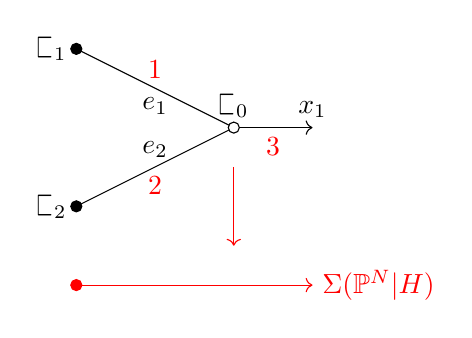
\begin{tikzpicture}
\draw [fill] (0,3) circle[radius=2pt];
\draw (0,3) node[left]{$\sqC_1$};
\draw (0,3) -- (2,2);
\draw (1,2.5) node[above,color=red]{$1$};
\draw (1,2.5) node[below]{$e_1$};

\draw [fill] (0,1) circle[radius=2pt];
\draw (0,1) node[left]{$\sqC_2$};
\draw (0,1) -- (2,2);
\draw (1,1.5) node[below,color=red]{$2$};
\draw (1,1.5) node[above]{$e_2$};

\draw [->] (2,2) -- (3,2);
\draw (3,2) node[above]{$x_1$};
\draw (2.5,2) node[below,red]{$3$};

\draw [fill=white] (2,2) circle[radius=2pt];
\draw (2,2) node[above]{$\sqC_0$};

\draw [->,color=red] (2,1.5) -- (2,0.5);

\draw [->,color=red] (0,0) -- (3,0);
\draw (0,0) [fill=red,color=red] circle[radius=2pt];
\draw (3,0) node[right,color=red]{$\Sigma(\PP^N|H)$};
\end{tikzpicture}
\end{center}
Here each edge (corresponding to a node of the curve) has a length $e_i$ and an expansion factor $u_i$ (indicated in red). The moduli space of such tropical maps is generated by the edge lengths $e_1$ and $e_2$
\begin{equation*} (\RR_{\geq 0})_{e_1} \times (\RR_{\geq 0})_{e_2} \end{equation*}
subject to the continuity condition $e_1=2e_2$. So the tropical moduli space is simply $\RR_{\geq 0}$ generated by $e_2$. Note that for any $e_2 > 0$ (i.e. on the interior of the cone) we have:
\begin{equation*} \lambda(\sqC_2) = e_2 = e_1/2 < e_1 = \lambda(\sqC_1). \end{equation*}
Thus, any logarithmic map with combinatorial type given by the above picture is automatically aligned. This means that the map $\VZ \to \Mcal$ is an isomorphism in a neighbourhood of our chosen element (there is no blowing up necessary). Indeed, the tropical moduli space is $\RR_{\geq 0}$ and this cone does not admit a polyhedral subdivision (there is no non-trivial toric blow-up of $\Aaff^1$).
\end{example}

\begin{example}
Consider now an element of $\Mcal$ whose associated tropical map has the corresponding combinatorial type:
\begin{center}
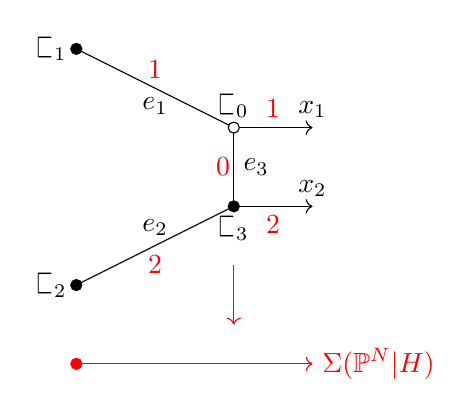
\begin{tikzpicture}
\draw [fill] (0,4) circle[radius=2pt];
\draw (0,4) node[left]{$\sqC_1$};
\draw (0,4) -- (2,3);
\draw (1,3.5) node[above,color=red]{$1$};
\draw (1,3.5) node[below]{$e_1$};

\draw [fill] (0,1) circle[radius=2pt];
\draw (0,1) node[left]{$\sqC_2$};
\draw (0,1) -- (2,2);
\draw (1,1.5) node[below,color=red]{$2$};
\draw (1,1.5) node[above]{$e_2$};

\draw [->] (2,3) -- (3,3);
\draw (3,3) node[above]{$x_1$};
\draw (2.5,3) node[above,red]{$1$};

\draw (2,3) -- (2,2);
\draw [fill] (2,2) circle[radius=2pt];
\draw (2,2.5) node[right]{$e_3$};
\draw (2.075,2.5) node[left,red]{$0$};
\draw (2,2) node[below]{$\sqC_3$};

\draw [->] (2,2) -- (3,2);
\draw (3,2) node[above]{$x_2$};
\draw (2.5,2) node[below,red]{$2$};

\draw [fill=white] (2,3) circle[radius=2pt];
\draw (2,3) node[above]{$\sqC_0$};

\draw [->,color=red] (2,1.25) -- (2,0.5);

\draw [->,color=red] (0,0) -- (3,0);
\draw (0,0) [fill=red,color=red] circle[radius=2pt];
\draw (3,0) node[right,color=red]{$\Sigma(\PP^N|H)$};
\end{tikzpicture}
\end{center}
As before, expansion factors are indicated in red and the edge lengths are $e_1,e_2,e_3$. The tropical moduli space is $\RR_{\geq 0}^3$ generated by these three lengths, subject to the continuity condition $e_1=2e_2$. Thus the moduli space is isomorphic to $\RR_{\geq 0}^2$ generated by $e_2$ and $e_3$. In order to have an alignment, at least one of $\lambda(\sqC_1)$ and $\lambda(\sqC_2)$ must be equal to the radius $\delta$. Note that
\begin{align*} \lambda(\sqC_1) & = e_1 = 2e_2 \\
\lambda(\sqC_2) & = e_2 + e_3\end{align*}
and without more information we cannot say which of these is larger. The subdivision of $(\RR_{\geq 0})^2$ is obtained by dividing the cone into regions where different order relations hold amongst the distances $\lambda(\sqC_1),\lambda(\sqC_2),\lambda(\sqC_3)$. The walls of this subdivison correspond to where some of these distances are equal. Note that in this setting we always have $\lambda(\sqC_2) > \lambda(\sqC_3)$ (at least, as long as we remain in the interior of the cone). The remaining possibilities are:
\begin{align*} \lambda(\sqC_1) & = \lambda(\sqC_3) \qquad (\Leftrightarrow e_1 = e_3 \Leftrightarrow 2e_2 = e_3) \\
\lambda(\sqC_1) & = \lambda(\sqC_2) \qquad (\Leftrightarrow e_1 = e_2 + e_3 \Leftrightarrow e_2 = e_3). \end{align*}
Thus, the subdivision of the tropical moduli space $(\RR_{\geq 0}^2)_{e_2 e_3}$ is given by:
\begin{center}
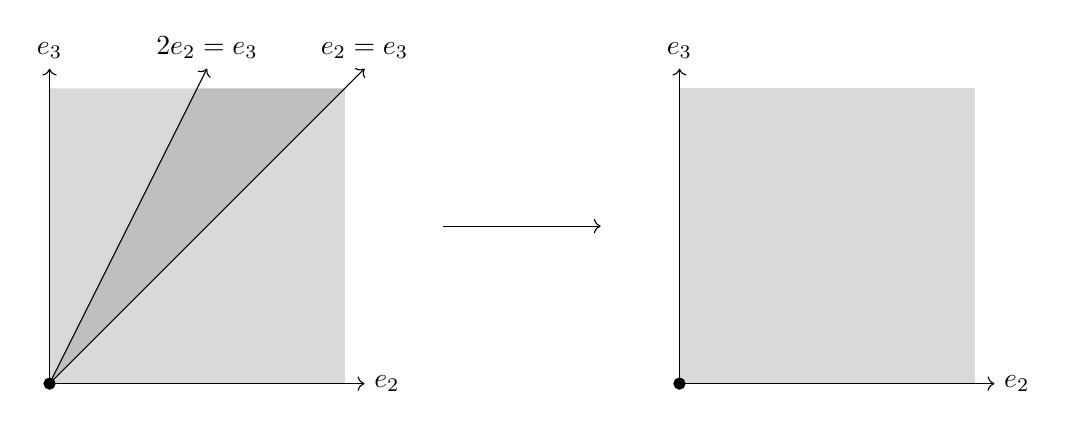
\begin{tikzpicture}[scale=1]
% Right-hand box
\fill [fill=gray!30!white] (5,0) -- (8.75,0) -- (8.75,3.75) -- (5,3.75) -- cycle;
\draw [fill] (5,0) circle[radius=2pt];
\draw [->] (5,0) -- (9,0);
\draw (9,0) node[right]{$e_2$};
\draw [->] (5,0) -- (5,4);
\draw (5,4) node[above]{$e_3$};

% Left-hand box
\fill [fill=gray!30!white] (-3,0) -- (0.75,0) -- (0.75,3.75) -- cycle;
\fill [fill=gray!50!white] (-3,0) -- (0.75,3.75) -- (-1.125,3.75) -- cycle;
\fill [fill=gray!30!white] (-3,0) -- (-1.125,3.75) -- (-3,3.75) -- cycle;
\draw [fill] (-3,0) circle[radius=2pt];
\draw [->] (-3,0) -- (1,0);
\draw (1,0) node[right]{$e_2$};
\draw [->] (-3,0) -- (-3,4);
\draw (-3,4) node[above]{$e_3$};

% 2e_2=e_3 line
\draw [->] (-3,0) -- (-1,4);
\draw (-1,4) node[above]{$2e_2=e_3$};

% e_2=e_3 line
\draw [->] (-3,0) -- (1,4);
\draw (1,4) node[above]{$e_2=e_3$};

% arrow
\draw [->] (2,2) -- (4,2);
\end{tikzpicture}
\end{center}
The cones of the subdivison index the logarithmic strata in a neighbourhood of the preimage in $\VZ$ of our chosen element of $\Mcal$. These can be described as follows:
\begin{center}
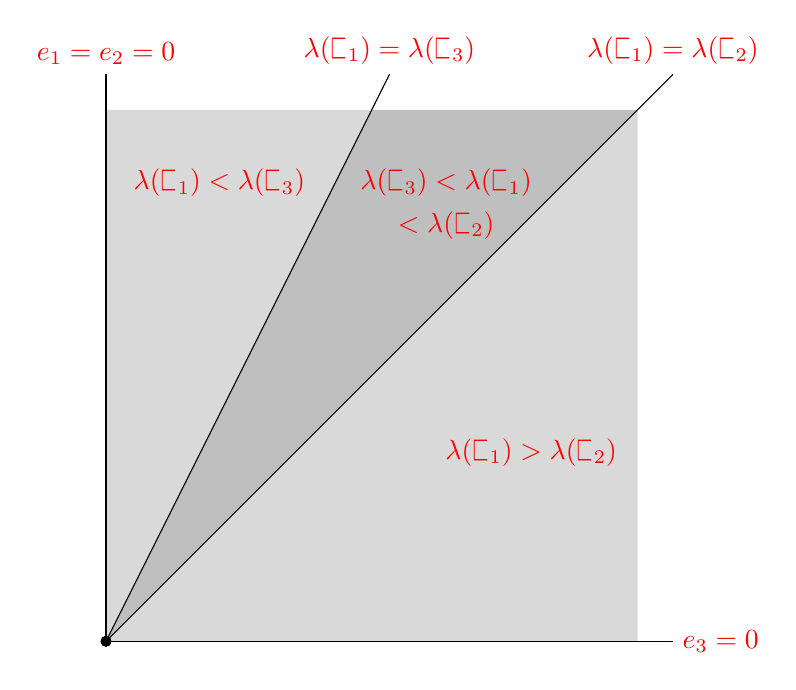
\begin{tikzpicture}[scale=1.8]
% Left-hand box
\fill [fill=gray!30!white] (-3,0) -- (0.75,0) -- (0.75,3.75) -- cycle;
\fill [fill=gray!50!white] (-3,0) -- (0.75,3.75) -- (-1.125,3.75) -- cycle;
\fill [fill=gray!30!white] (-3,0) -- (-1.125,3.75) -- (-3,3.75) -- cycle;
\draw [fill] (-3,0) circle[radius=1pt];
\draw (-3,0) -- (1,0);
\draw (1,0) node[right,red]{$e_3=0$};
\draw (-3,0) -- (-3,4);
\draw (-3,4) node[above,red]{$e_1=e_2=0$};

% 2e_2=e_3 line
\draw (-3,0) -- (-1,4);
\draw (-1,4) node[above,red]{$\lambda(\sqC_1)=\lambda(\sqC_3)$};

% e_2=e_3 line
\draw (-3,0) -- (1,4);
\draw (1,4) node[above,red]{$\lambda(\sqC_1)=\lambda(\sqC_2)$};

\draw (0,1.5) node[below,red]{$\lambda(\sqC_1) > \lambda(\sqC_2)$};

\draw (-0.6,3.4) node[below,red]{$\lambda(\sqC_3) < \lambda(\sqC_1)$};
\draw (-0.6,3.1) node[below,red]{$< \lambda(\sqC_2)$};

\draw (-2.2,3.4) node[below,red]{$\lambda(\sqC_1) < \lambda(\sqC_3)$};
\end{tikzpicture}
\end{center}
There are four codimension--$1$ logarithmic strata of $\VZ$ intersecting our chosen neighbourhood, corresponding to the rays in the above picture. Two of these -- those corresponding to the rays labeled $\{ e_1=e_2=0 \}$ and $\{ e_3=0 \}$ -- are the proper transforms of codimension--$1$ strata in $\Mcal$. These strata consist of log stable maps where some of the tropical edge lengths are equal to zero, meaning that the corresponding nodes have been smoothed. Notice that although the curve has three nodes, there are only two such strata: the nodes $q_1$ and $q_2$ cannot be smoothed independently because of the relation $e_1=2e_2$.

The remaining two codimension--$1$ strata in $\VZ$ -- corresponding to the interior rays in the above picture -- consist of log stable maps where some of the vertex distances become equal. Here none of the nodes are smoothed. From the construction of the subdivision, we see that both these strata map onto a codimension--$2$ stratum of $\Mcal$ (namely, the locus in which all of the nodes persist); this coheres with the fact that they should be thought of as exceptional loci of the blow-up. The extra dimension of moduli comes from the choice of alignment.

Finally, there are three codimension--$2$ strata, corresponding to different \emph{strict} orderings of the vertex distances. Note that the divisorial strata corresponding to $\{e_1=e_2=0\}$ and $\{e_3=0\}$, which intersected in $\Mcal$, no longer intersect in $\VZ$, since we have blown up. The picture is something like:
\begin{center}
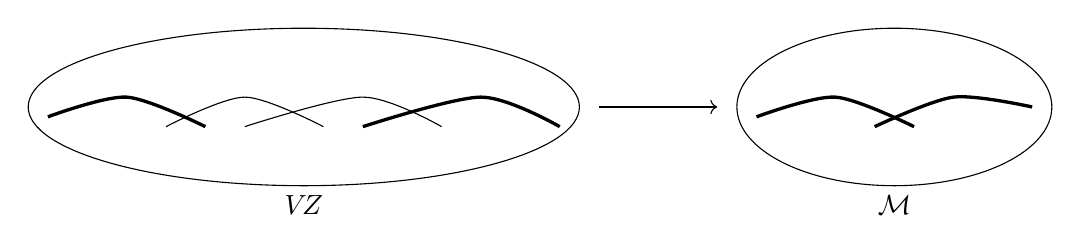
\begin{tikzpicture}[scale=0.5]
\draw (-6.5,0.5) ellipse (4 and 2);
\draw (-6.5,-1.5) node[below]{$\Mcal$};
\draw [very thick] plot [smooth] coordinates{(-10,0.25) (-8,0.75) (-6,0)};
\draw [very thick] plot [smooth] coordinates{(-7,0) (-5,0.75) (-3,0.5)};

\draw (-21.5,0.5) ellipse (7 and 2);
\draw (-21.5,-1.5) node[below]{$\VZ$};
\draw [very thick] plot [smooth] coordinates{(-28,0.25) (-26,0.75) (-24,0)};
\draw plot [smooth] coordinates{(-25,0) (-23,0.75) (-21,0)};
\draw plot [smooth] coordinates{(-23,0) (-20,0.75) (-18,0)};
\draw [very thick] plot [smooth] coordinates{(-20,0) (-17,0.75) (-15,0)};

\draw [->] (-14,0.5) -- (-11,0.5);
\end{tikzpicture}
\end{center}

\end{example}

\subsection{Global logarithmic strata}
In the previous subsections we used tropical geometry to identify the logarithmic strata of $\VZ=\VZ_{1,\alpha}(\PP^N|H,d)$ local to the preimage of a point in $\Mcal$. In fact, the whole discussion carries over if we replace a point in $\Mcal$ by a locally closed logarithmic stratum: the key observation is simply that the tropical moduli space does not vary if we move inside a locally closed logarithmic stratum, so the subdivision process makes sense over that whole stratum. This fact will allow us to describe the logarithmic strata of $\VZ$ globally.

\subsubsection{Logarithmic strata of $\Mcal$} The locally closed logarithmic strata of $\Mcal$ consist of loci where the combinatorial type of the associated tropical curve is constant\footnote{(Navid) Reference for this?}. This is because the combinatorial type determines the minimal monoid $Q$, which coincides with the stalk of the ghost sheaf on $\Mcal$.

If we have two strata $\Scal_1$ and $\Scal_2$ corresponding to combinatorial types $\Delta_1$ and $\Delta_2$, then $\Scal_2$ is contained in the closure of $\Scal_1$ if and only if the combinatorial type $\Delta_1$ is obtained from $\Delta_2$ by a process of generisation: namely, by contracting some edges (i.e. smoothing some nodes) and moving some of the vertices from the interior $\RR_{>0} \subseteq \RR_{\geq 0}$ of the tropicalisation $\Sigma(\PP^N|H)$ to the vertex $0 \in \RR_{\geq 0}$ (i.e. moving some components of the curve outside $H$). This allows us to completely describe the dual intersection complex of the logarithmic strata of $\Mcal$.

Note that we are \emph{not} able to easily read off the codimension of a logarithmic stratum from the combinatorial data: the codimension of the associated stratum in the Artin fan $\Acal_\Mcal$ is given by the dimension of the tropical moduli space, but the map $\Mcal\to\Acal_\Mcal$ is not smooth (since $\Mcal$ is not log smooth) so we are not able to say anything about the locus in $\Mcal$. 

\subsubsection{Logarithmic strata of $\VZ$}
Now let us pick a stratum $\Scal \subseteq \Mcal$ indexed by a combinatorial type $\Delta$ and with associated monoid $Q$. We may choose a sufficiently small open neighbourhood of $\Scal$ which only intersects logarithmic strata $\Scal^\prime$ which contain $\Scal$ in their closures. The previous discussion then shows that if we pick any point in this open neighbourhood, the combinatorial type of the associated tropical curve is obtained from $\Delta$ by contracting some edges and specialising some vertices. Thus we see that the associated map on tropical moduli spaces is injective, and so the generisation map on the level of ghost sheaves is surjective. This allows us to produce a chart on the open neighbourhood of $\Scal$ with monoid given by $Q$.

The discussion in the previous subsections then applies \emph{mutatis mutandis} to this open set, giving a description of the logarithmic strata of $\VZ$ which intersect an open neighbourhood of the preimage of $\Scal$. Since log strata must map to log strata, this gives a procedure for enumerating all of the locally closed logarithmic strata of $\VZ$, namely:\medskip
\begin{enumerate}
\item Enumerate the locally closed logarithmic strata of $\Mcal$ by enumerating all possible combinatorial types of tropical curves with the given numerical data. The dual intersection complex of these strata is specified by generisation of combinatorial types, as described earlier.\medskip
\item For each locally closed stratum $\Scal\subseteq \Mcal$ identify the tropical moduli space $Q^\vee_{\RR}$ associated to the given combinatorial type, and perform the subdivision specified by the alignment condition. The arguments of the previous subsections carry over to give a description of the logarithmic strata of $\VZ$ which map to a neighbourhood of $\Scal$. The dual intersection complex of these strata is specified by the combinatorics of each subdivision together with the dual intersection complex of the strata of $\Mcal$.
\end{enumerate}
We now illustrate this is in some examples:
\begin{example} Example of low-degree computation of logarithmic strata. (Note that for $\Mcal$ we can't read off the codimension from the dimension of the tropical moduli space because $\Mcal$ is not log smooth.)\footnote{(Navid) To be done.}\end{example}




\bibliographystyle{alpha}
\bibliography{Bibliography}

\bigskip\bigskip

\noindent Luca Battistella\\
Max-Planck-Institut f\"ur Mathematik, Bonn \\
\href{mailto:battistella@mpim-bonn.mpg.de}{battistella@mpim-bonn.mpg.de}\\

\noindent Navid Nabijou \\
School of Mathematics and Statistics, University of Glasgow \\
\href{mailto:Navid.Nabijou@glasgow.ac.uk}{navid.nabijou@glasgow.ac.uk}\\

\noindent Dhruv Ranganathan \\
DPMMS, University of Cambridge \\
\href{mailto:dr508@cam.ac.uk}{dr508@cam.ac.uk}

\end{document}